\chapter{MoE模型训练过程概述}

MoE模型在原本Transformer block的FFN中通过添加门控函数以及一系列相互并列的专家组成。
% 
在训练过程中门控函数主要将输入数据分配给不同的专家模型参与前向/反向计算,这一过程主要通过All-to-All通信实现。
% 
待每个专家计算完成相对应的数据之后,我们需要通过一次额外的All-to-All通信,将计算完成的激活值返回原本对应的GPU上,并参与后续的计算过程。

\section{MoE模型训练}

\begin{figure}[h!]
    \vskip 2ex
    \centering
    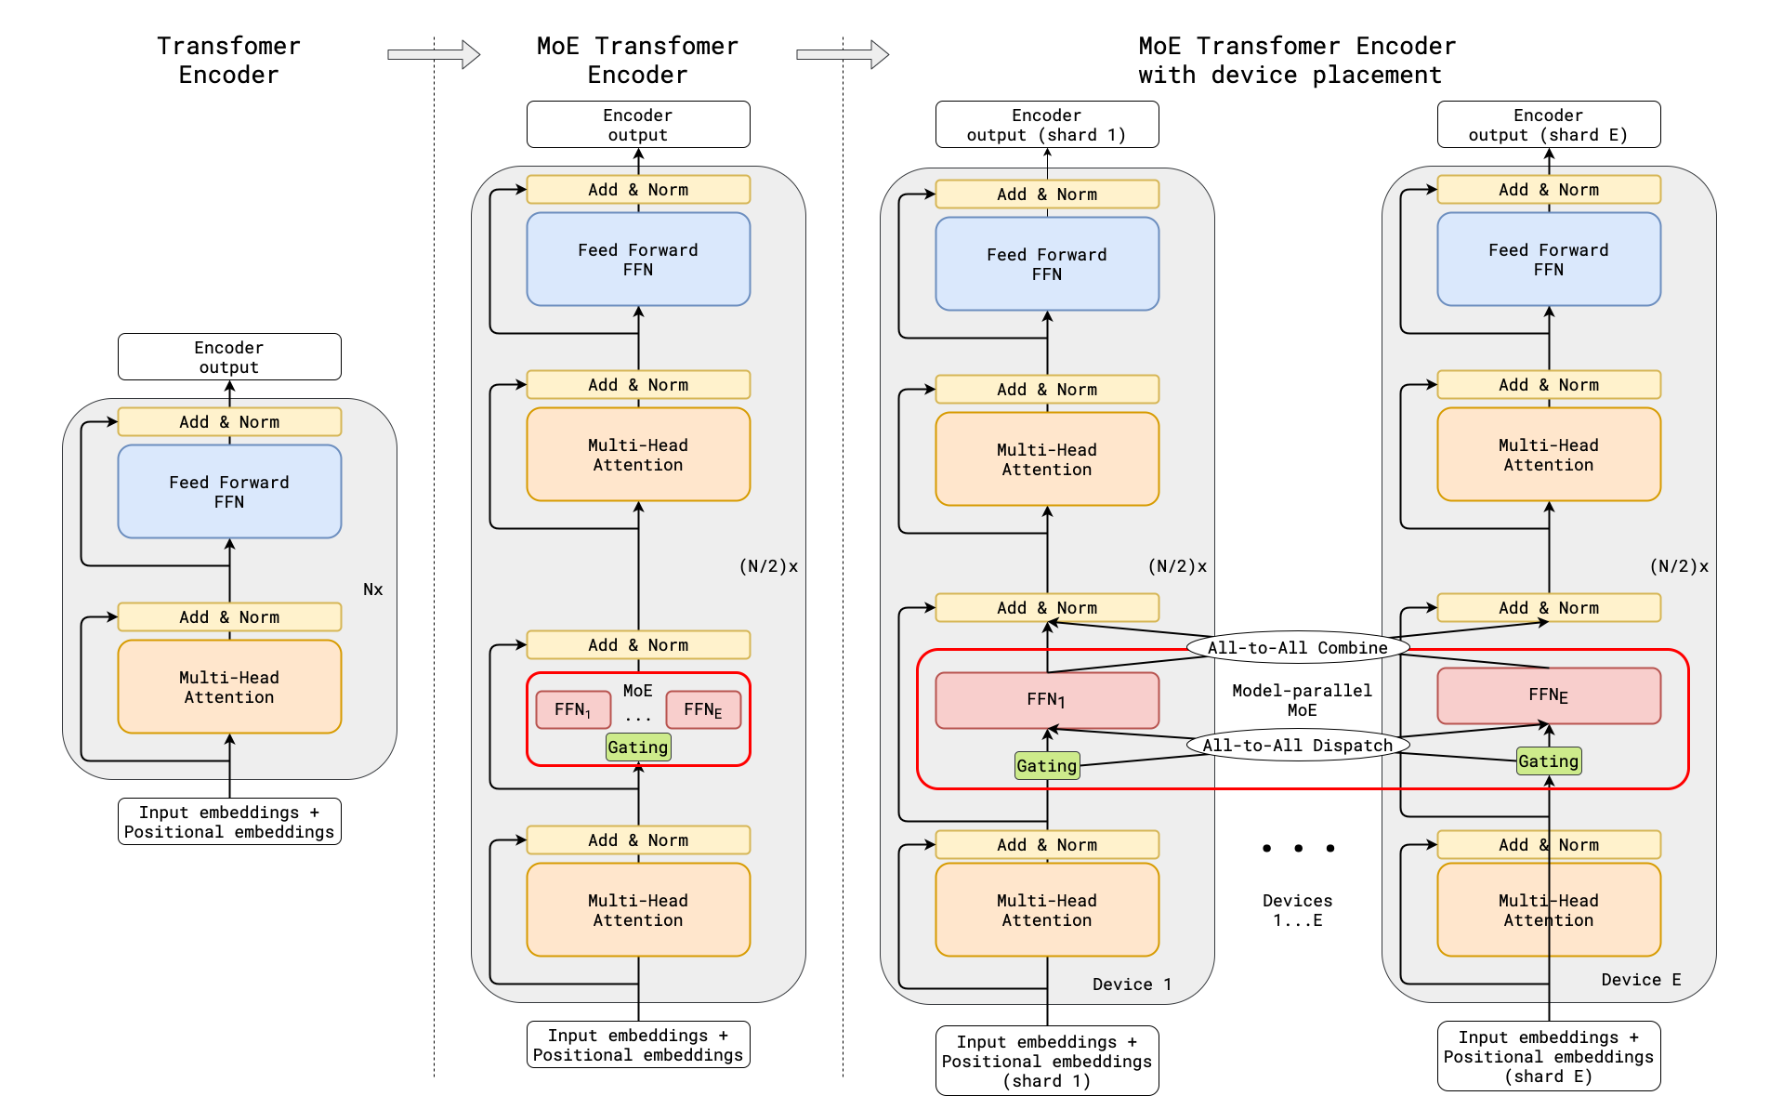
\includegraphics[width=0.99\linewidth]{figures/fig2.png}
    \caption{MoE模型训练过程}
    \label{fig-moe-arch}
    \end{figure}

图\ref{fig-moe-arch}展示了传统的集中式的Transformer模型训练过程转变到分布式的Transformer-MoE训练过程的示意图。
% 
绿色的部分是增加的门控函数,用于决定将数据分派至哪一个expert参与计算,红色部分的$\mathbf{FFN_1-FFN_E}$表示该层中具有E个互相独立的专家个数。
% 
由于GPU的显存有限,不能将所有的专家的参数都在一张GPU中保存下。
% 
因此GShard\ucite{lepikhin2020gshard}的研究者们提出了专家并行的概念,将每个专家的参数单独放置在GPU上,其他部分采用数据并行的架构,从而实现了一种混合的分布式训练过程。
% 
在训练过程结束之后,通常需要额外的All-reduce用于同步数据并行模块的梯度,最后根据每个可训练参数的梯度,调用优化器更新参数。

整体的训练流程总结如下:

\begin{itemize}

    \item \textbf{1.数据划分}
    
每个GPU将训练数据随机筛选,确保每一轮训练中每个GPU上包含的数据子集是互不重复的。
% 
每个子集分配到不同的GPU或计算节点上进行训练。
    
    \item \textbf{2.数据并行\&专家并行}
    
在MoE模型训练中,数据并行和专家并行通常结合使用,以实现更高效的分布式训练。
% 
具体而言,可以将训练数据划分为多个子集,并将每个子集分配到不同的GPU或计算节点上。
% 
在每个GPU或计算节点上,可以使用专家并行的方式对每个专家模型进行训练,同时使用数据并行的方式对整个MoE模型进行训练。
% 
这样可以将计算负载和数据负载都分散到多个GPU或计算节点上,从而加速整个MoE模型的训练过程。

    \item \textbf{3.前向传播}
    
    每一层的前向传播主要在以下两个步骤区别与传统的密集型Transformer计算。(数据分派和专家计算)。

在数据分派阶段,MoE模型使用Gating门函数对每个输入数据进行加权打分,以决定每个专家模型的贡献。这个Gating函数由一层MLP和softmax组成。具体而言,MoE模型将输入$x$输入到门控模型中,得到一个$E$维的得分,$f=[f_1,f_2,\cdots,f_E]$, $f_i$表示第$i$个专家模型的权重得分。门控向量的每个元素都是非负的,并且它们的和等于1,即$\sum_{i=1}^K g_i = 1$。最后通过全局所有GPU的All-to-All通信,将对应数据发送给相应的GPU,参与后续的计算。

专家计算阶段,每个GPU上接收到其他GPU传输来的数据后(假设有d维),将其输入相应的专家模型参与前向计算。
% 
得到d维的输出向量$r$。之后通过反向的All-to-All通信,将激活值返回对应的GPU上,得到每个GPU上原本数据的输出向量$z=[z_1,z_2,\cdots,z_E]$。
% 
然后,MoE模型将每个输出向量$z_i$与对应的门控向量$g_i$进行按元素乘法,得到一个加权输出向量$w$,其中$w_{i}=g_{i}z_{i}$。最后,MoE模型将所有加权输出向量$w_i$进行累加,得到最终的输出向量$y$,其中$y=\sum_{i=1}^E w_{i}$。

    \item \textbf{4.反向传播}
    
    是用于计算MoE模型的梯度,其过程类似于传统的神经网络模型。
    % 
    在完成前向传播计算之后,使用PyTorch的自动求导机制(autograd)建立计算图,并自动计算每个参数的梯度。
    % 
    具体而言,可以使用loss函数对模型的输出进行评估,并计算输出和目标值之间的误差。
    % 
    然后,使用误差及其对模型参数的导数,计算每个参数的梯度。
    % 
    反向传播过程可以使用链式法则(chain rule)实现,即将误差从输出层向输入层传播,并依次计算每个参数的梯度。

    \item \textbf{5.梯度计算}
    
    是将每个模型的梯度进行同步,以便在参数更新时使用。
    % 
    由于MoE模型的分布式训练过程涉及多个GPU或计算节点的并行计算,因此需要使用all-reduce等方法将所有模型的梯度进行同步。

    \item \textbf{6.参数更新}
    
    使用优化器对模型参数进行更新,以最小化损失函数。在MoE模型训练中,可以使用常见的优化器,如Adam、SGD等,对每个模型的参数进行更新。
    % 
    通常,参数更新的速率会受到学习率(learning rate)等超参数的控制,以平衡模型的收敛速度和稳定性。

    \item \textbf{7.重复迭代}
    
    将以上步骤重复多次,直到模型收敛为止。在每次迭代中,可以使用不同的训练数据子集,防止模型陷入局部最优解。

\end{itemize}

\section{本章小结}

本章我们主要分析了现有的MoE模型训练过程,MoE模型的训练过程通常比传统的神经网络模型更为复杂和耗时,需要充分利用分布式计算和并行计算等技术,以提高训练速度和效率。
% 
同时,MoE模型的设计和调整也需要考虑多个因素,如门控模型的设计、专家模型的选择和训练方式等,以提高模型的性能和泛化能力。

\endinput